%With increased precision of data, the calculations must also progress to higher accuracy, involving an increased number of diagrams with each 
%additional order, and this translates into computationally demanding 
%calculations even for the DIS processes. Such calculations 
%are too slow to be used iteratively in a fit.
%There are several methods available which allow fast PDF extractions.  
%Two such techniques
%are implemented into \fitter: the $k$-factor approximation from lower to higher order in theoretical precision and the fast grid techniques using interfaces to the 
%packages \texttt{fastNLO} \rm and \texttt{APPLGRID}. These techniques are briefly described below.  
%\\
More precise measurements
require theoretical predictions with equally improved accuracy in
order to maximize their impact in PDF fits.  Perturbative
calculations, however, get more and more involved with increasing
number of Feynman diagrams at the each higher order. 
Nowadays even the most advanced perturbative techniques in
combination with recent computing hardware do not lead to sufficiently
small turn-around times. The direct inclusion of computationally
demanding higher-order calculations into iterative fits therefore is
not possible. Relying on the fact that a full repetition of the
perturbative calculation for arbitrary changes in input parameters is
not necessary at each iteration step, two methods have been developed
to resolve this problem: the techniques of $k$-factors and
\emph{fast grids}. Both are available in \fitter and described as follows.

%\begin{description}
%\item{\bf$k$-factor technique:}
\subsection{$k$-factor Technique}
  The $k$-factors are defined as the ratio of the prediction of a
  higher-order (slow) pQCD calculation to a lower-order (fast)
  calculation. Because the $k$-factors depend on the phase space
  probed by the measurement they have to be stored into a table in
  dependence of the relevant kinematic variables. Before the start of
  a fitting procedure the table of $k$-factors has to be computed once
  for a given PDF with the time consuming higher-order code. In
  subsequent iteration steps the theory prediction is derived from the
  fast lower-order calculation multiplied by the pre-tabulated
  $k$-factors.

  However, this procedure neglects the fact that the $k$-factors are
  process dependent and, 
%  and are, for example, different for dijet
%  production from quark-quark or gluon-gluon initial states. 
  as a consequence, they have to be re-evaluated
  for the newly determined PDF at the end of the fit in order to check
  for any changes. Usually, the fit is repeated until input and output
  $k$-factors have converged. In summary, this technique avoids to
  iterate the higher-order calculation at each step, but still
  requires a couple of repetitions depending on the analysis.


\begin{itemize}
%\item For the DIS process, the heavy flavour schemes provide accurate but computationally slow calculations. 
%In \fitter ``FAST'' schemes were implemented 
%such that the $k$-factors used can be
%the ratio between same order calculations but massive versus massless
%i.e. NLO (ACOT)/NLO (ZM-VFNS), or 
%the ratio between NLO (massive)/LO (massless).
%The $k$-factors are only calculated for the PDF parameters at the first 
%fit iteration
% and hence, the FAST heavy flavour schemes should only be used 
%for quick checks and the full scheme is recommended.
%%%%
%The method was employed in the QCD fits to the HERA data when ACOT scheme was used as a cross check of the central results \cite{h1zeus:2009wt}, as shown in Fig.~\ref{fig:acotrt}.
%
  \item In DIS, appropriate treatments of the heavy quarks require  
    computationally slow calculations.
    For this purpose, ``FAST'' heavy flavour schemes are implemented
    in \fitter with $k$-factors defined as the ratio of
    calculations at the same perturbative order but for massive vs.\
    massless quarks, e.g.\ NLO (massive)/NLO (massless).
    In the \fitter
    implementation, these $k$-factors are calculated only for the
    starting PDF and hence, the ``FAST'' heavy flavour schemes should
    only be used for quick checks, i.e. full heavy flavour schemes
    are recommended. For ACOT case,
    %and it is recommended to apply the full heavy flavour schemes 
    due to long computation time, the $k$-factors are used in 
    the default settings in \fitter.  Fig.~\ref{fig:acotrt} illustrates
    the PDFs extracted from  the QCD fits to the HERA data, for which 
     the ``FAST'' method for ACOT was used as a cross check to the main results ~\cite{h1zeus:2009wt}.

\begin{figure}[!ht]
\centering
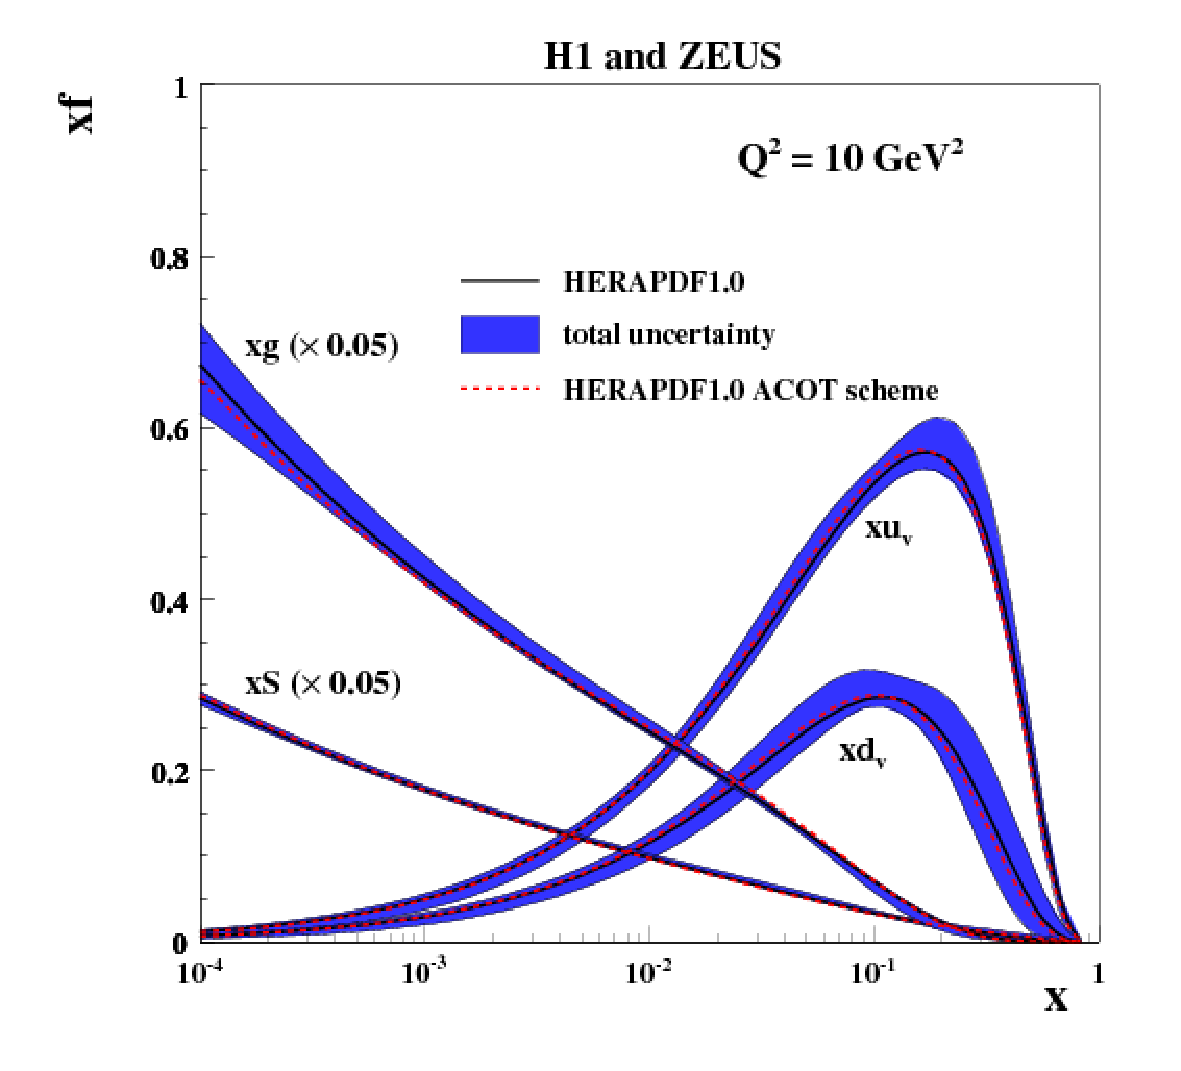
\includegraphics[width=8cm]{heraacot}
  \caption{Overview showing the $u-$ and $d$-valence, the total sea
    (scaled), and gluon (scaled) PDFs of the NLO HERAPDF1.0 set \cite{h1zeus:2009wt} 
    with their 
    total uncertainty at the scale of $Q^2 = 10\ \GeV^2$ obtained 
    using the TR' scheme and compared to the PDFs obtained with 
    the ACOT scheme using the $k$-factor technique (red).}
 \label{fig:acotrt}
\end{figure}



%\item 
%In the case of the DY processes the LO calculation described in section~\ref{dysection}
%is such that the PDFs can be factorised, allowing high speed calculations when 
%performing QCD fits over lepton rapidity data. In this case
%the factorised part of the expression which is independent of PDFs can be
%calculated only once for all minimisation iterations.
%The leading order code in \fitter package implements this 
%optimisation and uses fast convolution routines provided by
%\qcdnum. Currently the full width LO calculations are optimised 
%for lepton pseudorapidity and boson rapidity distributions with the
%possibility to apply lepton \(p_{\perp}\) cuts.
%making this procedure flexible to describe data.
%This flexibility allows the calculations to be performed within the phase space
%corresponding to the available measurement.
%The calculated LO cross sections are multiplied by
%$%k$-factors to obtain predictions at NLO.
%
%  \item In the case of the DY process a part of the LO calculation
%    described in Section~\ref{dysection} can be factored out such that
%    high speed calculations become possible when performing QCD fits
%    with lepton rapidity data. The part of the expression that can be
%    written as an extra factor is independent of the PDFs and needs to
%    be derived only once for all minimisation iterations. The
%    leading-order code in \fitter implements this optimisation and
%    uses fast convolution routines provided by \qcdnum. Currently, the
%    full width LO calculations are optimised for lepton pseudorapidity
%    and boson rapidity distributions with the possibility to apply
%    selection criteria to the lepton \pperp.
%    % making this procedure flexible to describe data.
%    This flexibility allows to perform the computations for
%    the phase space corresponding to each available measurement.
%    % The calculated leading order cross sections are multiplied by
%    % NLO or NNLO k-factors provided for corresponding data
%    % distributions.
%    The LO cross sections are then multiplied by $k$-factors to
%    obtain predictions at NLO\@.

\end{itemize}


%\vspace*{0.25cm}
%\item{\bf{}Fast grid technique:}
\subsection{Fast Grid Techniques}

  Fast grid techniques exploit the factorisable nature of the cross sections and 
  the fact that iterative PDF fitting
  procedures do not impose completely arbitrary changes to the types
  and shapes of the parameterised functions that represent each PDF\@.
  Instead, it can be assumed that a generic PDF can be approximated by
  a set of interpolating functions with a sufficient number of
  strategically well-chosen support points. The quality, i.e.\ the
  accuracy of this approximation, can be tested and optimised by a
  number of means, the simplest one being an increase in the number of
  support points. Ensuring an approximation bias that is negligibly
  small for all practical purposes this method can be used to perform
  the time consuming higher-order calculation (see Eq.~\ref{eq:fact})
  only once for the set of interpolating functions. 
  The repetition of a cross section evaluation for
  a particular PDF set then is very fast and implies only sums over
  the set of interpolators multiplied by factors depending on the
  respective PDF\@. The described approach applies equally to
  processes involving one or two hadrons in the initial state as well
  as to the renormalisation and factorisation scale dependence in the
  convolution of the PDFs with the partonic cross section.

  This technique was pioneered in the \fastnlo
  project~\cite{Kluge:2006xs} to facilitate the inclusion of
  notoriously time consuming jet cross sections at NLO into PDF fits.
  The \applgrid~\cite{Carli:2010rw} package extended first a similar
  methodology to DY production. While differing in their interpolation
  and optimisation strategies, both packages construct tables with
  grids for each bin of an observable in two steps: In the first step
  the accessible phase space in the parton momentum fractions $x$ and
  the renormalisation and factorisation scales \mur and \muf is
  explored in order to optimize the table size. The second step
  consists of the actual grid construction and filling for the
  requested observables. Higher-order cross sections can then be
  restored very efficiently from the pre-produced grids while varying
  externally provided PDF sets, \mur and \muf, or the strong coupling
  \asq\@. The approach can in principal be extended to arbitrary
  processes, but requires to establish an interface between the
  higher-order theory programs and the fast interpolation
  frameworks. Work in that direction is ongoing for both packages.
  They are described in some more detail in the following:

\begin{itemize}
  \item The \fastnlo project~\cite{Kluge:2006xs} has been interfaced
    to the \nlojetpp program~\cite{Nagy:1998bb} for the calculation of
    jet production in DIS~\cite{Nagy:2001xb} as well as 2- and 3-jet
    production in hadron-hadron collisions at
    NLO~\cite{Nagy:2003tz,Nagy:2001fj}. To demonstrate the
    applicability to higher-orders, threshold corrections at 2-loop
    order, which approximate the NNLO for the inclusive jet cross
    section, have been included into the framework as
    well~\cite{Wobisch:2011ij} following Ref.~\cite{Kidonakis:2000gi}.
    % KR: Maybe not necessary to include in a HERAFitter document
    % Recently it was shown~\cite{Kumar:2013hia,deFlorian:2013qia},
    % however, that in particular for the LHC the jet size $R$
    % dependence must be taken into account in these threshold
    % corrections.

    The latest version of \fastnlo~\cite{Britzger:2012bs} allows 
    creation of tables where renormalisation and factorisation scales
    can be chosen
    freely as a function of two pre-defined observables, e.g.\ jet
    transverse momentum \pperp and $Q$ for DIS\@. 
    \fastnlo can be obtained from~\cite{fastNLO:HepForge}, where
    numerous pre-calculated grid tables for jet cross sections can be
    downloaded as well. 
%    The latest release is compatible with \lhapdf
%    versions 5 or 6, includes the \as evolution package
%    \crundec~\cite{Schmidt:2012az}, and can also be linked to use the
%    \hoppet or \qcdnum evolution. The C++ library part can be accessed
%    via an optional Python interface.

    Dedicated \fastnlo libraries and tables required for comparison to
    particular datasets are included in the \fitter package. In this
    case, the evaluation of the strong coupling constant is taken
    consistently with the PDF evolution from the \qcdnum code. The
    interface to the \fastnlo tables from within \fitter was used in a
    recent CMS analysis, where the impact on the
    extraction of the PDFs from the inclusive jet cross section is
    investigated~\cite{cms:jets}. The influence on the gluon density by
    the CMS inclusive jet data is illustrated in Fig.~\ref{fig:cmsjet}.

\begin{figure}[!ht]
  \centering
  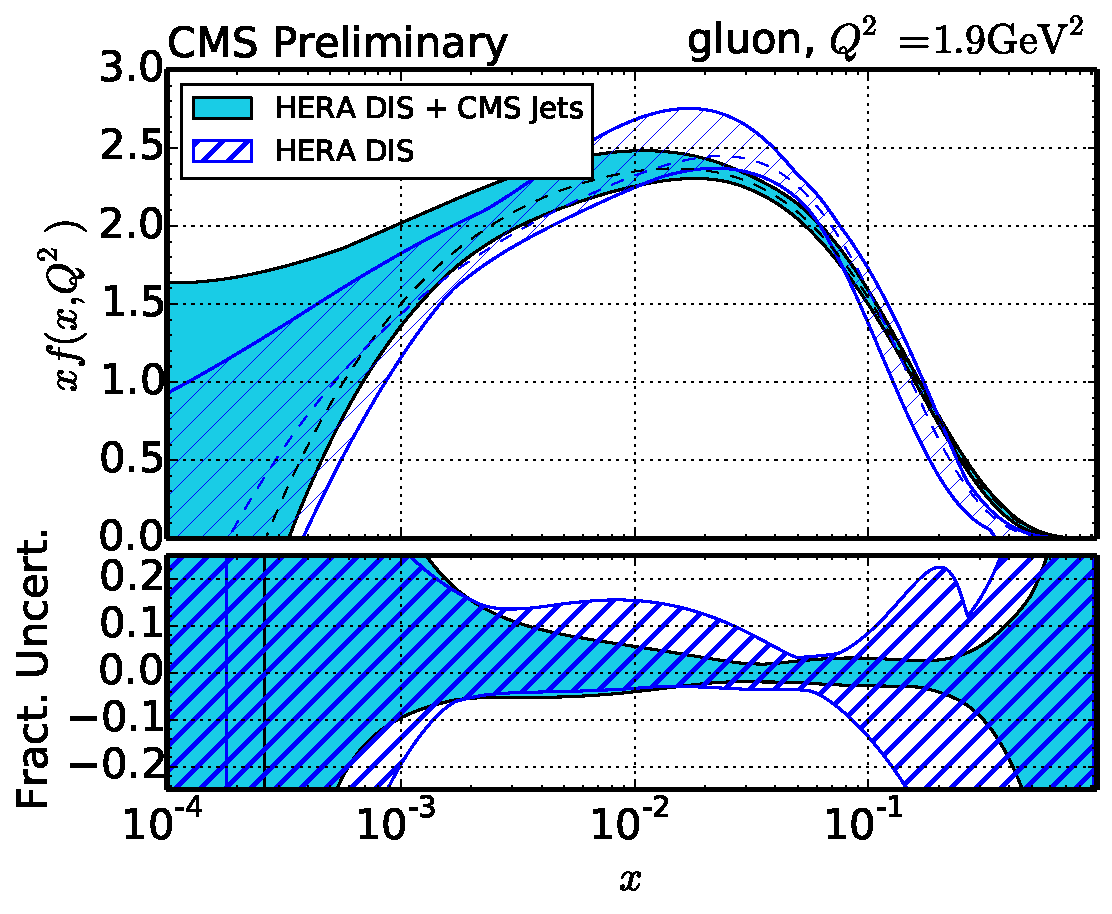
\includegraphics[width=8cm]{CMSjets}
  \caption{The gluon density as a function of $x$ as derived from
    HERA inclusive DIS data alone (cyan) and in combination with
    CMS inclusive jet data from 2011 (blue hatched) \cite{cms:jets}, 
    where bands
    represent the total uncertainty of the PDFs. The PDFs are
    shown at the starting scale $Q^2 = 1.9\ \GeV^2$.}
  \label{fig:cmsjet}
    \end{figure}

\item The \applgrid package~\cite{Carli:2010rw}, which is also
    available from~\cite{APPLGRID:HepForge}, in addition to
    the jet cross sections from \nlojetpp 
    in $pp(\bar p)$ and DIS processes, implements the calculations 
    of DY production. The look-up tables (also called grids) can be generated with
    modified versions of the \mcfm parton level generator for
    DY~\cite{Campbell:1999ah,Campbell:2000je,Campbell:2010ff}.  
%    The cross section observables and the grid parameters are 
%    defined in the \applgrid code.
    Alternative values of the strong coupling constant as well as 
    a posteriori variation of the renormalisation 
    and factorisation scales can be freely chosen in the calculation
    of the theory predictions with the \applgrid tables. 
    For NNLO predictions in \fitter $k$-factors can be applied.

    The \fitter interface to \applgrid was used by the ATLAS
    collaboration to extract the strange quark density of the proton
    from $W$ and $Z$ cross sections~\cite{atlas:strange}. An
    illustration of ATLAS PDFs extracted using the $k$-factors is shown in
    Fig.~\ref{fig:atlas} together with the comparison to global PDF
    sets CT10~\cite{CT10pdf} and NNPDF2.1~\cite{NNPDFpdf}.

\begin{figure}[!ht]
  \centering
  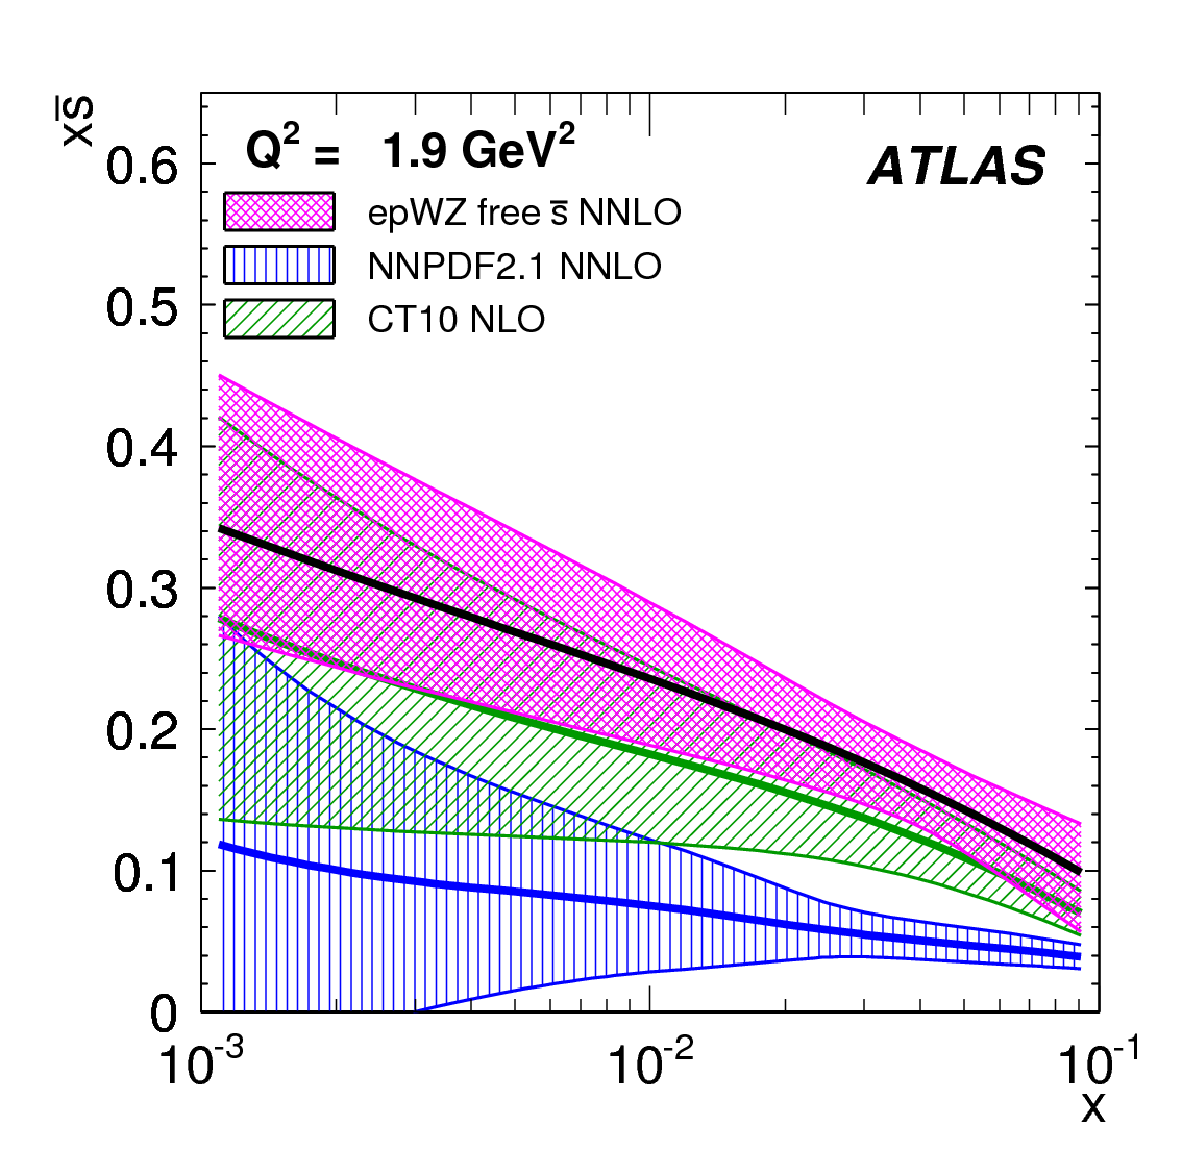
\includegraphics[width=8cm]{atlas.pdf}
  \caption{The strange anti-quark density versus $x$ for the ATLAS
    epWZ free sbar NNLO fit (magenta band) compared to predictions
    from NNPDF2.1 (blue hatched) and CT10 (green hatched) 
    at $Q^2 = 1.9\ \GeV^2$. The ATLAS fit was performed using $k$-factor method 
    for NNLO corrections. The figure is taken from \cite{atlas:strange}.}
  \label{fig:atlas}
\end{figure}

%    \item The \applgrid~\cite{Carli:2010rw} package allows the fast computation 
%of NLO cross sections for particular processes for arbitrary sets of 
%proton parton distribution functions. The package implements
%calculations of DY production as well as jet production in $pp(\bar p)$
%collisions and DIS processes. 
%
%The approach is based on storing the perturbative coefficients
%of NLO QCD calculations of final-state observables measured
%at hadron colliders in look-up tables. The PDFs and the 
%strong couplings are included during the final calculations,
%e.g. during PDF fitting. The method allows 
%variation of factorisation and renormalisation scales in
%calculations.
%
%The look-up tables (grids) can be generated with modified versions
%of the \texttt{MCFM} parton level generator for DY~\cite{Campbell:1999ah,Campbell:2000je,Campbell:2010ff} 
%or \nlojetpp~\cite{Nagy:1998bb,Nagy:2001fj} code for NLO jet production.
%The model input parameters are pre-set as usual for \texttt{MCFM}, 
%while binning and definitions of the
%cross section observables are set in the \applgrid code.
%%as distributed with the full version of APPLGRID package.
%% NLO calculations
%%for the current analysis are performed with the help of APPLGRID
%%generated grids based on MCFM calculations. 
%%
%%APPLGRID supports an interface to the MCFM parton level generators,
%%hence model input parameters such as electroweak parameters
%%are in fact pre-set following the MCFM input steering card, while
%%binning and definitions of the observables for which the
%%differential cross sections are needed are set in the 
%%APPLGRID code. 
%%The grid parameters \(x_1, x_2\) and \(Q^2\) binning
%The grid parameters, \(Q^2\) binning
%and interpolation orders are also defined in the code.
%
%\applgrid constructs the grid tables in two 
%steps: {\it (i)} exploration of the phase space in order
%to optimize the memory storage and {\it (ii)} actual grid
%construction in the phase space corresponding to the 
%requested observables.
%The NLO cross sections are restored from the grids
%using externally provided PDFs, $\as$, factorization and 
%renormalization scales. For NNLO predictions $k$-factors can be applied.
%
%This method was used by the ATLAS collaboration in determining the strange 
%quark density of the proton from $W$ and $Z$ cross sections 
%together with HERA inclusive DIS data~\cite{atlas:strange}. 
%An illustration of PDFs extracted in~\cite{atlas:strange} using \applgrid method 
%and $k$-factors to correct from NLO to NNLO is shown 
%in Fig.~\ref{fig:atlas} together with the comparison to the global PDF sets 
%CT10~\cite{CT10pdf} and NNPDF2.1~\cite{NNPDFpdf}.
%
%\begin{figure}[!ht]
%   \centering
%   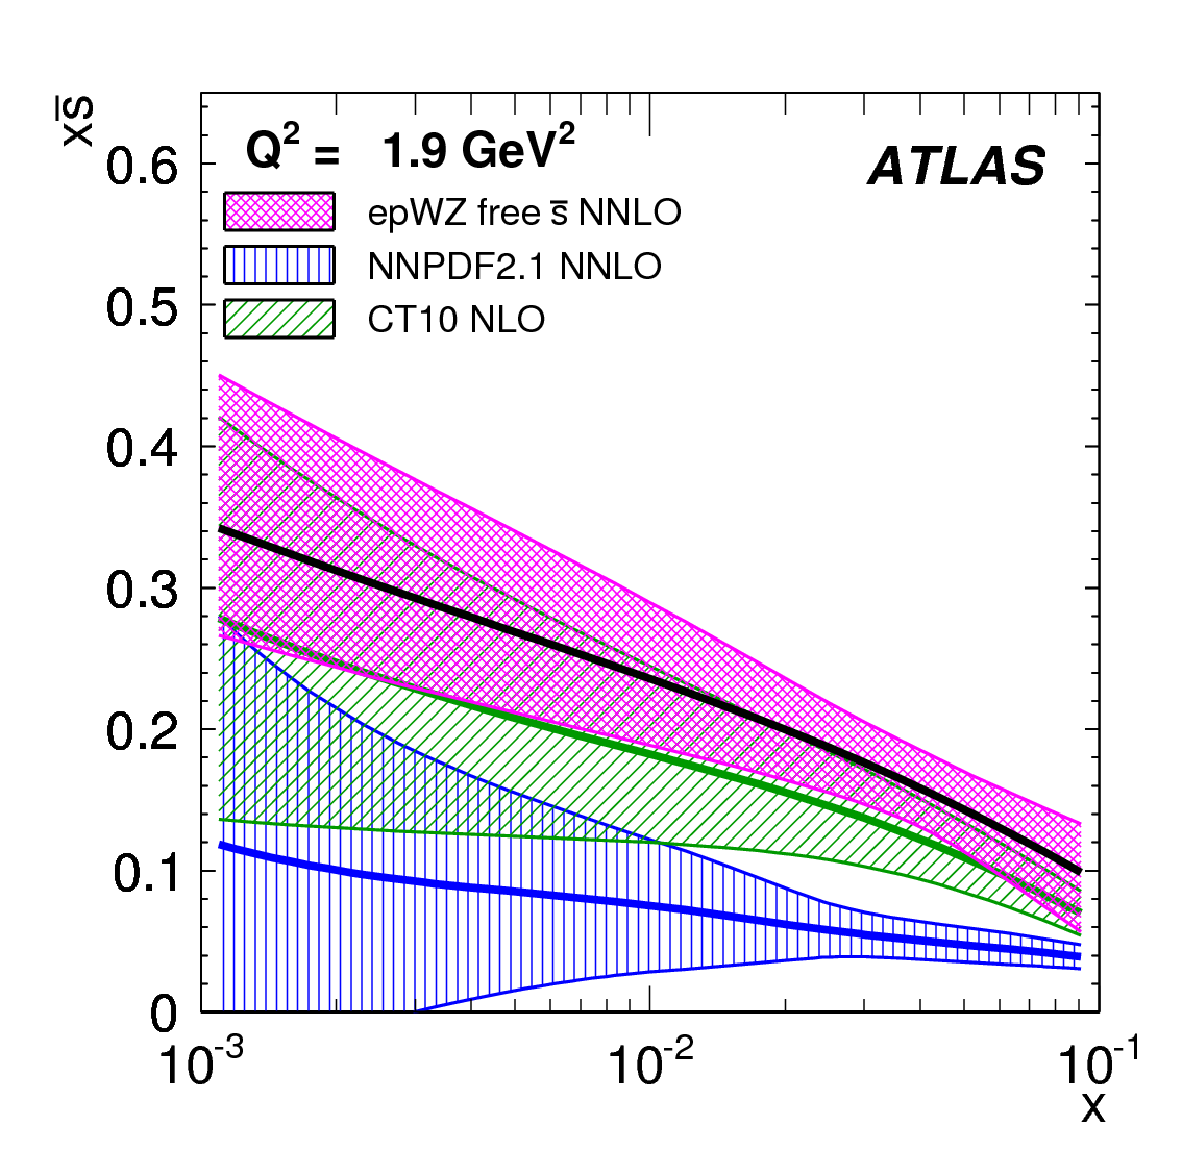
\includegraphics[width=8cm]{atlas.pdf}
%   \caption{The strange anti-quark density versus $x$ for the ATLAS epWZ free sbar NNLO fit (magenta band) compared to predictions from NNPDF2.1 (blue hatched) and CT10 (green hatched) at $Q^2= 1.9 \ \GeV^2$.}
% \label{fig:atlas}
%\end{figure}
%
%

\end{itemize}

%\end{description}

%\subsection{Performance Optimisation}
%
%An important factor for a feasible QCD fit which is performed by iterative 
%$\chi^2$ minimisation, is performance in terms of how long a calculation takes for each given data point.
%The performance of the \fitter code is greatly improved with several special built-in options
%including the $k-factor$ techniques (see section~\ref{sec:techniques}) and the grid techniques for the fast calculation of cross 
%sections of particular processes for arbitrary sets of PDFs. There are also cache options, fast evolution kernels, and 
%usage of the OpenMP (Open Multi-Processing) interface which allows
%parallel applications of some of the heavy flavour scheme theory predictions in DIS. 


